\apendice{Documentación técnica de programación}

\section{Introducción}
En este apéndice se va a realizar una descripción más avanzada del proyecto, para aquella persona que desee continuar su desarrollo o conocer el funcionamiento más a fondo.

\section{Estructura de directorios}
En esta sección vamos a dar un sentido a la organización de las carpetas del trabajo.

\begin{itemize}

\item\textbf{algorithms:} En este directorio vamos a encontrar todos los algoritmos realizados a lo largo del proyecto, dos ficheros son el algoritmo de backpropagation y el encargado de hacer el cálculo de rachas,el resto tienen una nomeclatura particular:
\begin{itemize}
\item Scraping: Los ficheros que empiezan  así,son los ficheros utilizados para el web scraping.
\item Informe: Estos scripts son los encargados de mostrarnos por la interfaz las tablas correspondientes.
\end{itemize}
\item\textbf{database:} Contiene la última versión de la base de datos.

\item\textbf{images:} Este directorio tiene las imágenes que se muestran en la interfaz.

\item\textbf{otros:} El resto de directorios son propios de Drupal, apenas se han hecho cambios en estos ya que no ha sido necesario. En el directorio sites/all/themes, se ha añadido el tema de bootstrap que podemos observar en la interfaz
\end{itemize}

\section{Manual del programador}

En esta sección vamos a ver diversas acciones que nos van a permitir un uso más avanzado del trabajo desarrollado.

Para el manejo de la interfaz web, es necesario un cierto conocimiento de uso del gestor Drupal.

\subsection{Administración interfaz web}
PAra la dministración de la misma, lo primero es logearse como administrador en Drupal, para ello hay que acceder a la página de login:
\begin{lstlisting}[language=html,keywordstyle=\color{black}]
http://localhost/?q=user/login
\end{lstlisting}
\begin{figure}
\centering
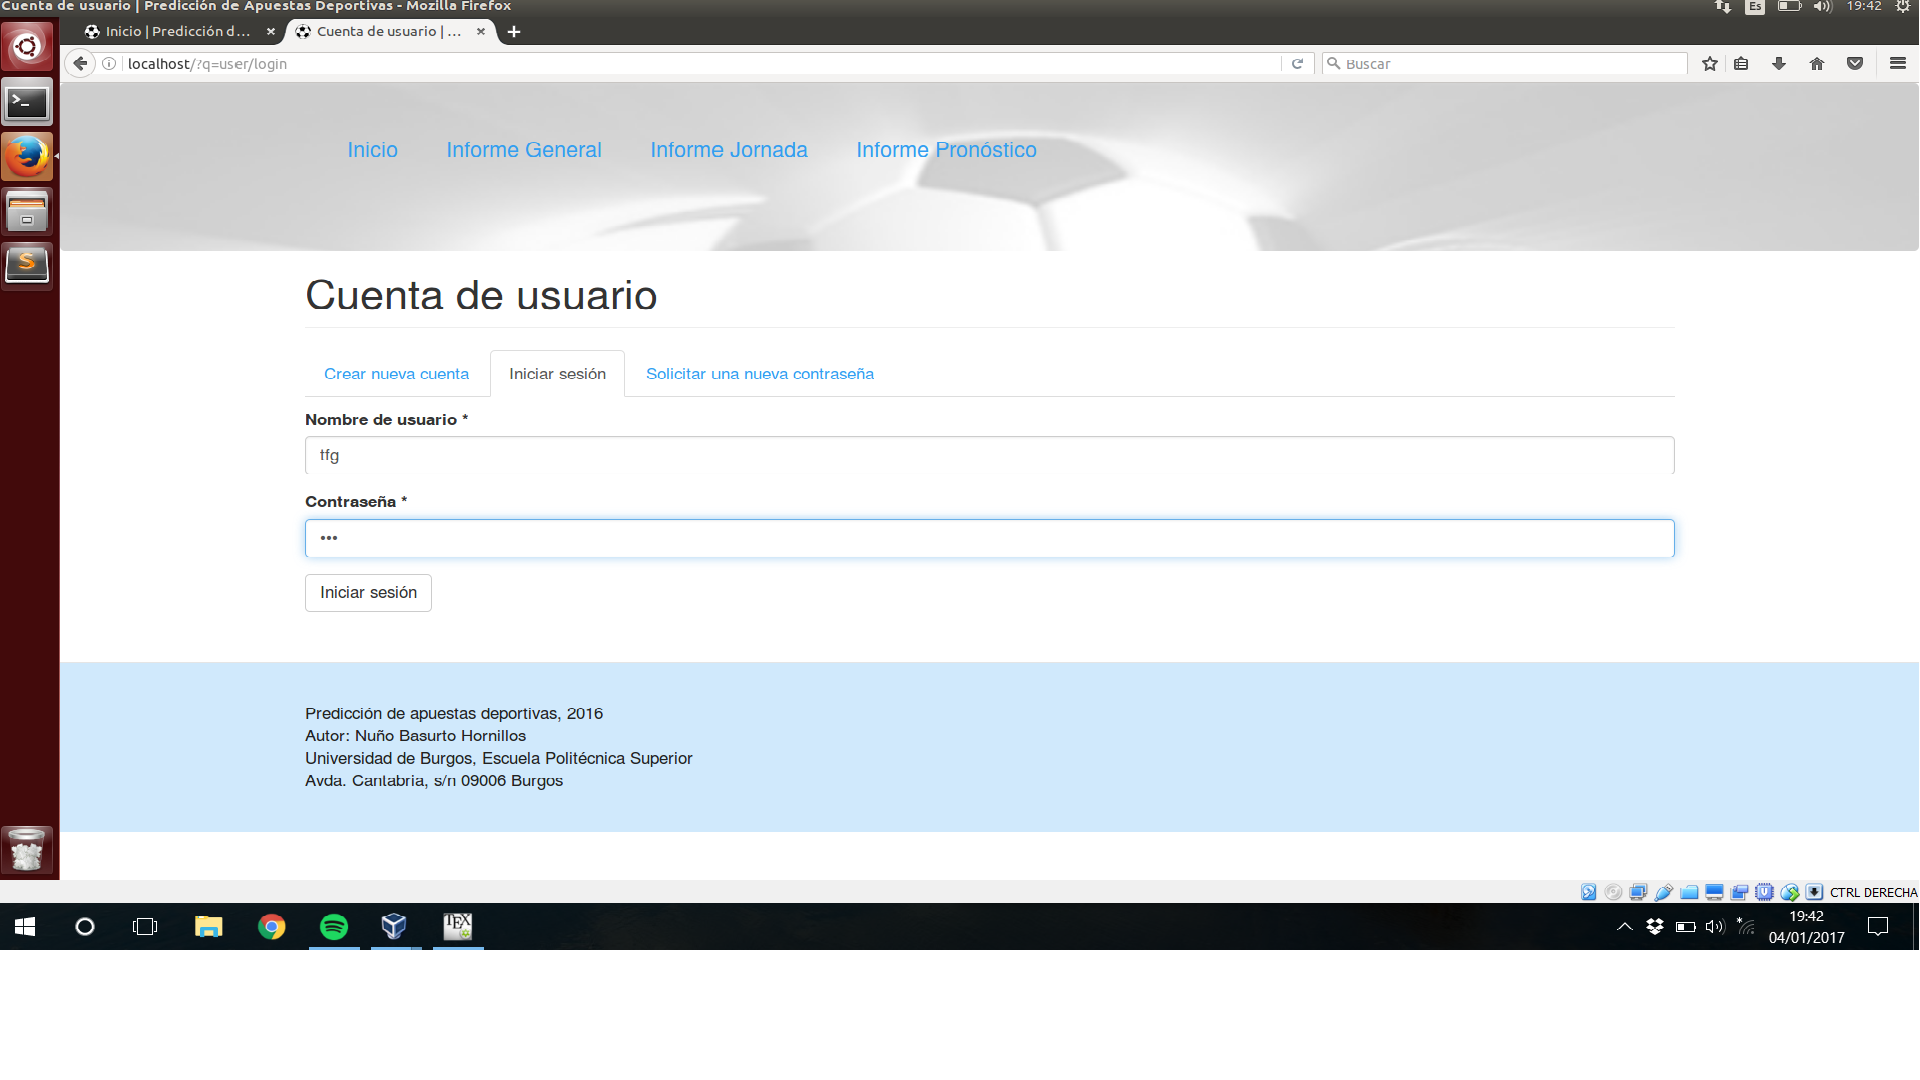
\includegraphics[width=.9\textwidth]{img/drupal_login}
\caption{Loguearse en Drupal}
\label{fig:AdminAp}
\end{figure}
Introducimosel usuario \textit{tfg} y la contraseña \textit{tfg}. Una vez dentro si queremos ejecutar algún algoritmo, por que por ejemplo en el momento de ejecución del demonio el servidor no estaba activo, accederemos al panel de la izquierda llamado Navegación y pulsaremos en Administrar apuestas, aquí nos mostrará los diferentes posibilidades de ejecución
\begin{figure}
\centering
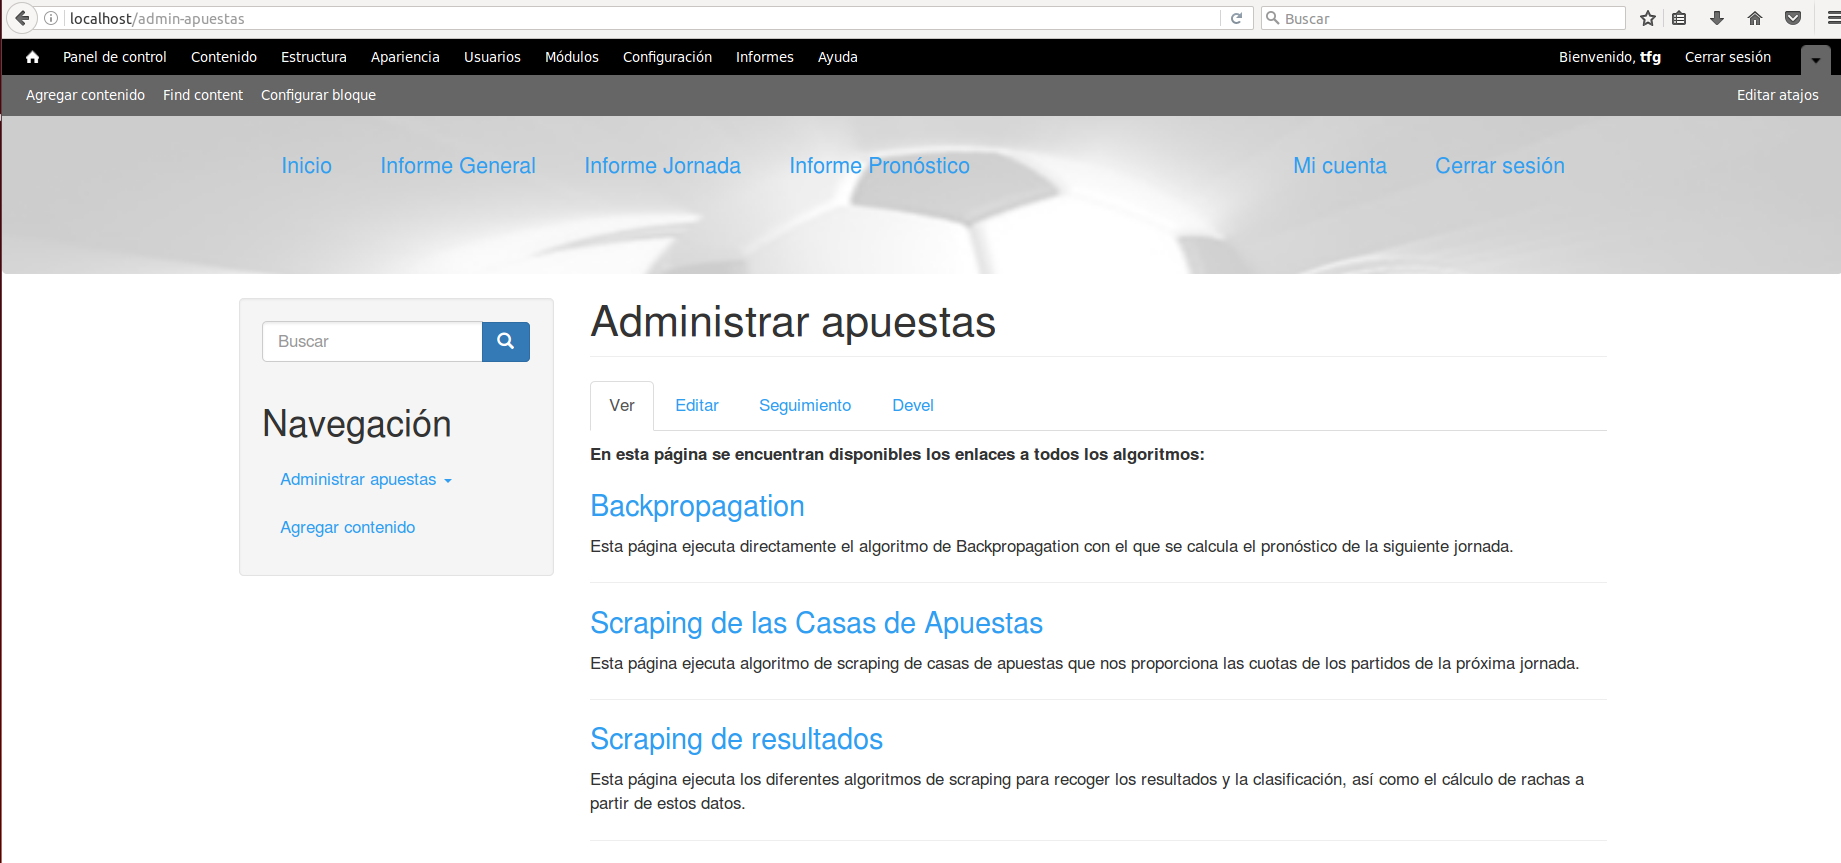
\includegraphics[width=.9\textwidth]{img/drupal_admin_apuestas}
\caption{Administración de apuestas}
\label{fig:AdminAp}
\end{figure}

En la parte de arriba en un color grisáceo oscuro tenemos los atajos\ref{fig:AtajDru}, el primero <<Agregar contenido>> nos permite añadir nuevas páginas donde ejecutar algoritmos, find content nos permite realizar ejecuciones, modificaciones o eliminar los contenidos ya existentes\ref{fig:FindCont}. Si por ejemplo deseamos editar un fichero, en este caso \textit{Scraping de resultados}, nos encontramos con este código: 
\begin{figure}
\centering
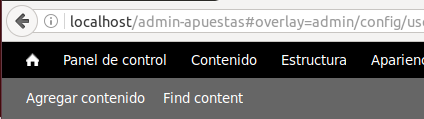
\includegraphics[width=.9\textwidth]{img/drupal_atajos}
\caption{Atajos en Drupal}
\label{fig:AtajDru}
\end{figure}
\begin{figure}
\centering
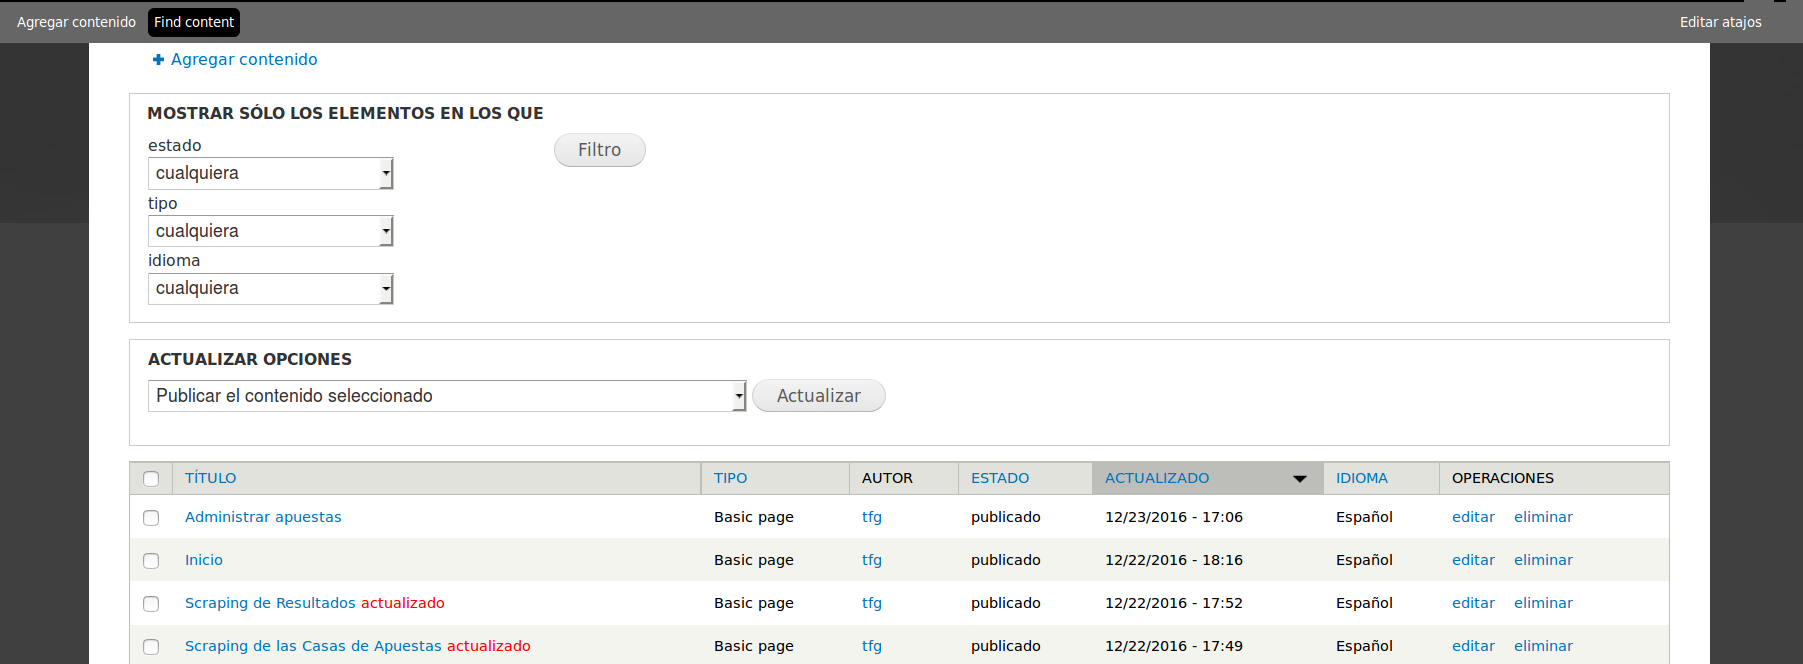
\includegraphics[width=.9\textwidth]{img/drupal_find_content}
\caption{Editar contenidos}
\label{fig:FindCont}
\end{figure}
\begin{lstlisting}[language=php,keywordstyle=\color{black}]
<?php
include_once 'algorithms/Scraping_resultados.php'
include_once 'algorithms/Scraping_clasificacion.php'
include_once 'algorithms/Calculo_rachas.php'
?>
\end{lstlisting}
De esta sencilla manera llama a los algoritmos que deseamos, ahora toca añadir unas líneas especiales dentro de los scripts, para que Drupal pueda acceder a ellos:
\begin{lstlisting}[language=php,keywordstyle=\color{black}]
define('DRUPAL_ROOT', getcwd());
require_once DRUPAL_ROOT . '/includes/bootstrap.inc';
drupal_bootstrap(DRUPAL_BOOTSTRAP_FULL);
\end{lstlisting}
Está hecho de esta forma para no tener que copiar todo el código del script, en el contenido de Drupal. De esta forma se puede utilizar un buen editor de código fuente, como Sublime Text, en vez de usar el editor de texto de Drupal que complica mucho y ralentiza la programación.

Este ha sido un pequeño resumen de como realizar las modificaciones básicas en Drupal, si se desea aprender más a fondo las modificaciones que se pueden realizar, es recomendable el libro [DRUPAL 7 - Bibliografia] y ante dudas acudir a la comunidad de Drupal, que expone sus dudas en \url{https://www.drupal.org/forum}.

\section{Compilación, instalación y ejecución del proyecto}
En esta sección se va a hablar de aquellos pasos que hay que llevar a cabo para poder trabajar sobre el el proyecto y la implementación del código.

La instalación va a realizarse sobre la distribución de Linux Ubuntu, en concreto sobre su versión 14.04. Bien puede realizarse sobre una máquina virtual o como anfitrión.
\subsection{LAMP}
LAMP es el acrónimo de la infraestructura de internet que trabaja con las siguientes herramintas:
\begin{itemize}
\item Linux: Como sistema operativo.
\item Apache: El servidor web.
\item MySQL: Como gestor de base de datos, aunque también puede instalarse MariaDB
\item PHP: Lenguaje de programación,  aunque también esta aceptado el uso de Perl y Python.
[Referencia LAMP Wikipedia]
\end{itemize}
\subsubsection{Apache}
El primer paso va a ser la instalación del servido web Apache en nuestro sistema. El servidor puede ser instalado perfectamente a través de la shell de Linux:
\begin{lstlisting}[language=bash,keywordstyle=\color{black}]
$ sudo apt-get update
$ sudo apt-get install apache2
\end{lstlisting}
Una vez realizado esto ya tenemos el servidor instalado, para comprobar que funciona correctamente entramos en el navegador y ponemos: 
\begin{lstlisting}[language=bash,keywordstyle=\color{black}]
http://localhost
\end{lstlisting}
Tras ello deberíamos ver:
\begin{figure}
\centering
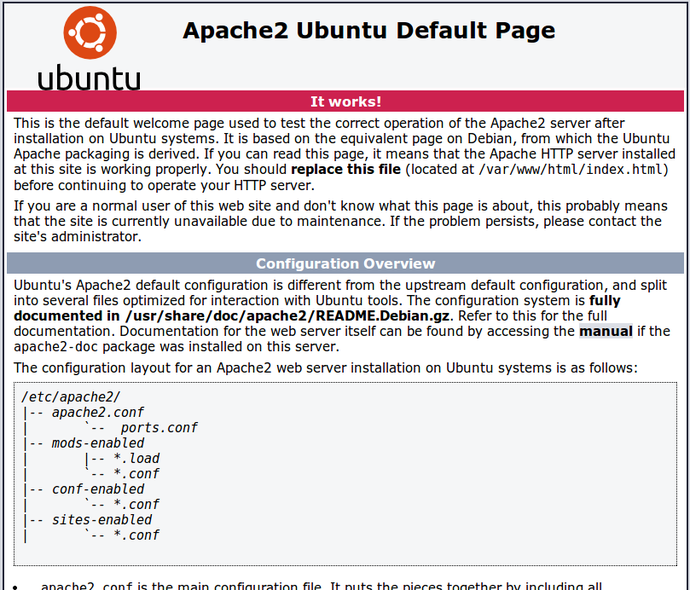
\includegraphics[width=.9\textwidth]{img/apache}
\caption{Apache en funcionamiento}
\label{fig:Apache}
\end{figure}

\subsubsection{MySQL}
Ahora vamos a proceder a instalar el gestor de bases de datos MySQL, para ello   escribimos en el terminal el siguiente comando:
\begin{lstlisting}[language=bash,keywordstyle=\color{black}]
$ sudo apt-get install mysql-server mysql-client
\end{lstlisting}
Es una instalación sencilla, debemos recordar la contraseña y el usuario utilizados.
Ahora vamos a proceder a crear la base de datos en MySQL y  seguidamente un script de seguridad.
\begin{lstlisting}[language=bash,keywordstyle=\color{black}]
$ sudo mysql_install_db
$ sudo mysql_secure_installation
\end{lstlisting}
\subsubsection{PHP}
Lo primero es instalar PHP y para ello vamos a ejecutar el siguiente comando en la terminal:
\begin{lstlisting}[language=bash,keywordstyle=\color{black}]
$ sudo apt-get install libapache2-mod-php5 php5 php5-mcrypt
\end{lstlisting}
Tras ello procedemos a intalar algunos módulos de PHP:
\begin{lstlisting}[language=bash,keywordstyle=\color{black}]
$ sudo apt-get install php5-cgi php5-cli php5-common php5-curl php5-dbg php5-dev php5-gd
\end{lstlisting}
Podemos comprobar que se ha instalado correctamente creando el fichero:
\begin{lstlisting}[language=bash,keywordstyle=\color{black}]
$ sudo nano/var/www/html/info.php
\end{lstlisting}
Insertándole el código:
\begin{lstlisting}[language=PHP,tabsize=4,frame = single,caption=Código par comprobar el funcionamiento de PHP''. ,captionpos=b,label=lst:pruebaPHP]
<?php
	phpinfo();
?>
\end{lstlisting}
Finalmente en el navegador ponemos: 
\begin{lstlisting}[language=html,keywordstyle=\color{black}]
http://localhost/info.php
\end{lstlisting}
La imagen que nos encontremos debería ser similar a esta:
\begin{figure}
\centering
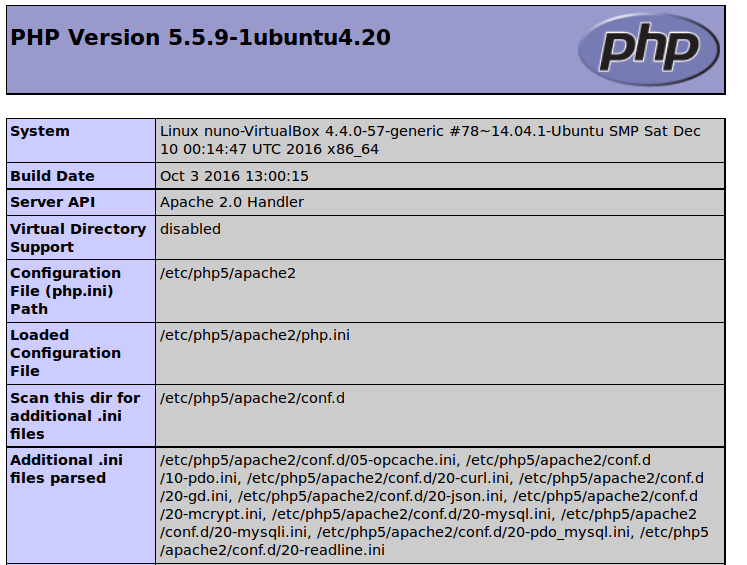
\includegraphics[width=.9\textwidth]{img/php}
\caption{Instalación PHP}
\label{fig:php}
\end{figure}

Ahora tenemos que activar el módulo de PHP para Apache, para ello en el fichero
\begin{lstlisting}[language=bash,keywordstyle=\color{black}]
$sudo nano /etc/apache2/mods-enabled/php2.conf
\end{lstlisting}
Hay que cambiar la línea a On.
\begin{lstlisting}[language=bash,keywordstyle=\color{black}]
php_admin_value engine On
\end{lstlisting}
Tras el cambio es muy importante reinicia el servicio de apache así:
\begin{lstlisting}[language=bash,keywordstyle=\color{black}]
$ sudo service apache2 restart
\end{lstlisting}

\subsection{phpMyAdmin}
Una vez instalado LAMP, vamos a instalar el gestor de MySQL phpMyAdmin, que nos va a ayudar a trabajar en la base de datos. Lo primero es instalar su paquete:
\begin{lstlisting}[language=bash,keywordstyle=\color{black}]
$ sudo apt-get install phpmyadmin
\end{lstlisting} 
En el paso de la instalación que pregunta por la utilización de dbconfig-common hay que indicar <<yes>>. Tras ello habilitamos la extensión php5-mcrypt:
\begin{lstlisting}[language=bash,keywordstyle=\color{black}]
$ sudo php5enmod mcrypt
\end{lstlisting}
Una vez realizados estos apsos reiniciamosel servicio apache como hicimos anteriormente:
\begin{lstlisting}[language=bash,keywordstyle=\color{black}]
$ sudo service apache2 restart
\end{lstlisting}
Tras ello ya podemos acceder a través del navegador con:
\begin{lstlisting}[language=html,keywordstyle=\color{black}]
http://localhost/phpmyadmin
\end{lstlisting}

\subsection{Drupal 7}

Lo primero es descargarse la última versión de Drupal 7 de la página \url{http://www.drupal.org}, decargamos sobre la raíz del sistema. Una vez esté este fichero en la raíz al poner la url en el navegador: \url{http://localhost/admin}, nos encontraremos con una interfaz con la cual la instalación de Drupal nos resultará bastante sencilla.
En la primera pantalla escogemos que queremos un perfil Standard y continuamos. Más adelante nos pediré el nombre de la base de datos, es necesario que esta exista ya en nuestro servidor para que Drupal pueda ser instalado. Y de esta manera sencilla nos encontramos con Drupal 7 instalado.

Una vez instalado Drupal 7 podemos seleccionar diferentes módulos y temas para añadir al gestor de contenido. En el desarrollo de este proyecto se intentó trabajar con algunos módulos como el de Trello pero este tenía problemas con la autentificación. En cambio si que se instaló satisfactoriamente el tema de Bootstrap con el cual nos encontramos en la interfaz. Para instalar un tema es aconsejable descargarlo desde \url{http://www.drupal.org/project/project_theme} y tras ello descomprimirlo en la carpeta \textit{/sites/all/themes} tras ello si accedemos en nuestro navegador a la dirección: \url{http://localhost/admin/appearance} nos lo encontraremos así, para los módulos es similar, solo que hay que almacenar el módulo descargado y descomprimido en \textit{/sites/all/modules} y tras ello acceder a la página \url{http://localhost/admin/modules}.

\section{Pruebas del sistema}

Dado que hemos realizado un diseño web centrado en el usuario es necesario realizar una serie de pruebas centradas en el usuario. Se ha realizado a un total de 10 usuarios con la edad comprendida entre los 22 y 56 años.

Las pruebas se realizaron con fecha de 27 de Diciembre de 2016. La última jornada disputada era la 16 y la que estaba pronosticada era la 17. Se propusieron una serie de cuestiones en un orden determinado y se observaron las acciones de los usuarios.

\begin{itemize}
\item Acceder al pronóstico de la próxima jornada. \textbf{9/10}
\item Acceder al balance global de todas las jornadas. \textbf{10/10}
\item Obtener el balance global de la jornada 14 de BET365. \textbf{10/10}
\item Acceso al balance de la última jornada.\textbf{7/10}
\item Acceder al balance de la jornada 14. \textbf{5/10}
\end{itemize}

Con este sencillo test nos hemos encontrado con la dificultad de algunos usuarios para acceder al balance de una jornada particular y es que, para este acceso los usuarios debían acceder a \textit{Informe Global} y desde ahí pichar en la jornada correspondiente, dado que los usuarios estaban en la página \textit{Informe Jornada}, buscaban algún enlace desde la jornada que ahí teníamos y la jornada 14.

Las conclusiones extraídas del test nos indican la necesidad de poner enlaces en \textit{Informe Jornada} al resto de jornadas, para evitar volver a \textit{Informe Global}. En cuanto al resto del sitio web al ser sencillo apenas genera problemas al usuario.

